\section{Sparsity in DNN Training}
 \label{sec:sparse_dnn_training}
 
 In this section we motivate our work and project the benefits of our optimizations for DNN training.  First, we provide some intutition of why sparsity exists in DNN training.  Next, using an image recogntion workload, we empirically demonstrate the amount of sparsity that exists in practice.  Finally, we discuss how available sparsity can be exploited using our techniques to improve training efficiency. 
 
\subsection{Sources of Sparsity}
\label{subsec:sparsity_source}

Machine learning experts have long observed that DNN training using back-propagation and gradient descent involves a considerable amount of computations on sparse matrices and vectors~\cite{Ng04, Nair10, Krizhevsky12, Bengio13, Srivastava14a}.  The performance-critical data of training are neuron activations and errors (both implemented as vectors) and synaptic weights and corresponding deltas (both implemented as matrices) can be sparse.  Some of the sparsity arise naturally from the training process and its matrix-vector multiplication kernel.  For example, correct predictions of a neuron's output activation, during feed-forwad evaluation, result in zero-valued neuron error terms, during back-propagation, which can introduce sparsity in the rest of the network.  Beyond this, standard techniques for boosting training quality often introduce additional sparsity in the network.  These include techniques such as Rectified Linear Units (ReLUs)~\cite{Nair10, Krizhevsky12} for faster convergence, and  L$_1$~\cite{Ng04, Bengio13} and Dropout~\cite{Srivastava14a} regularization methods for reducing overfitting.  {\color{red} Trishul to help with this content}
 
\begin{figure*}
 \centering
 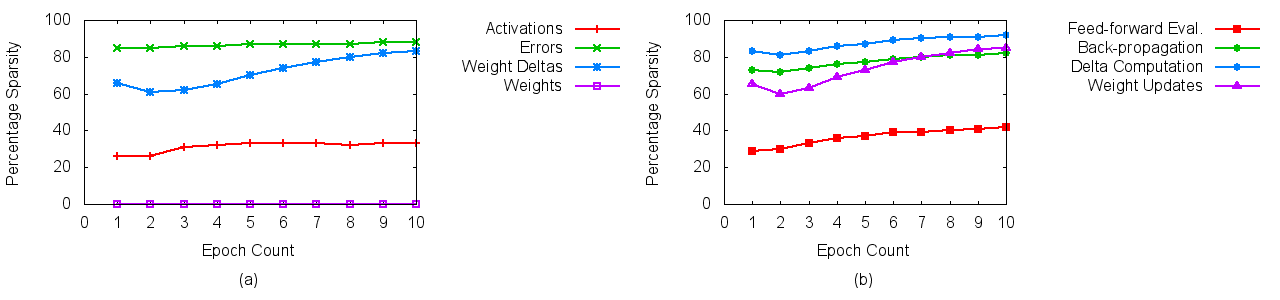
\includegraphics[width=1.9\columnwidth]{Figures/cifar-10_word_sparsity.png}
\caption{(a) Data and (b) computation sparsity in CIFAR-10 training.}
 \label{fig:cifar-10_word_sparsity}
 \end{figure*}

\subsection{Sparsity in real-word image recognition task}
\label{subsec:sparsity_profile}

For a better insight into the amount of sparsity in real-world DNN training workloads, we profile training on {\it CIFAR-10}~\cite{KrizhevskyThesis}, a standard image recognition task (described in ~\ref{subsec:eval_method}).  In our study, we reason about sparsity from $2$ perspectives: (i) data sparsity and (ii) computation sparsity.  Specifically, data sparsity measures the amount of zeroes in performance-critical data (e.g., activation vectors), while computation sparsity measures the amount of mutiply-accumulate operations performed on zero values in the main phases of training (e.g., feed-forward evaluation).  Both perspectives are useful because they capture different effects of sparsity on system performance.  Memory capacity bandwidth impact is captured by data sparsity, processing cycles impact is captured by computation sparsity, and bandwidth impact is captured by both data and computation sparsity.  We measure both sparsity metrics over $10$ training epochs using a data set of $60000$ images. 

\subsubsection{Data Sparsity.} 

Figure~\ref{fig:cifar-10_word_sparsity}(a) illustrates the sparsity of activation and error vectors, and weight delta and weight matrices in CIFAR-10 training.  We see that the sparsity amount and rate of change is quite different among the data structures.  While the weight matrix is dense, the activation and error vectors and the weight delta matrix are noticeably sparse.  We see that sparsity generally increases with training epochs, albeit at varying rates.  The error vector has the greatest amount of sparsity ($83\%$---$85\%$), followed by the weight delta matrix ($66\%$---$83\%$), and finally the activation vector ($26\%$---$33\%$).  The results show the memory/cache consumption of activations, errors, and weight deltas for this workload can be reduced significantly. 

\subsubsection{Computation Sparsity.}
 Figure~\ref{fig:cifar-10_word_sparsity}(b) reports the computation sparsity of the different training steps. Compared to data sparsity, the results illustrate how the different vectors and matrices are combined through multiplication and addition operations.  For example, the sparsity in feed-forward evaluation is the result of multiplying the dense weight matrix and sparse activation vector.  We see that considerable sparsity exists in each training step (from $29\%$ for feed-forward evaluation to $92\%$ for computing weight deltas).  We also see that the amount of sparsity generally grows with training epochs (e.g., $29\%$---$42\%$ for feed-forward evalution).  In summary, these results shows the potential for significant saving in processing cycles by eliminating cycle consumption for generating zero values that do not impact training quality.  

\begin{figure*}
 \centering
 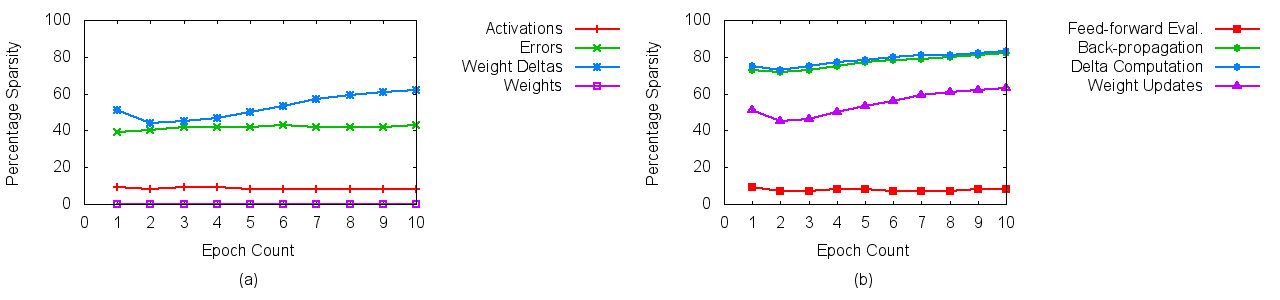
\includegraphics[width=1.9\columnwidth]{Figures/cifar-10_cacheline_sparsity.png}
\caption{(a) Data and (b) computation sparsity in CIFAR-10 training at cacheline granularity.}
 \label{fig:cifar-10_cacheline_sparsity}
 \end{figure*}

\subsection{Sparsity at cache line granularity}
\label{subsec:sparse_opt_limit}

Our proposed hardware mechanisms track data sparsity at cache line granularity, so it is unlikely that we can fully exploit the amounts of sparsity presented above because the profiling was conducted at a finer granularity (e.g., individual activation values). To get a more accurate view of  the effectiveness of our optimizations we repeat the profiling study at a cache line granularity. Since data values are represented as 4-byte floats (or word), each cache line contains up to $16$ data values. We measure sparsity at cache line granularity in the following manner.  Data sparsity represents the percentage of cache lines of a data structure that contain only zero values.  For computation, we adopt a coarse-grained veiw of computations, i.e., a unit of computation operates on a pair of cache lines (e.g., an activation cache line and a weight cache line in feed-forward evaluation).  Thus,  computation sparsity represents the percentage of such computations that operate on a sparse cache line. The results are presented in Figures~\ref{fig:cifar-10_cacheline_sparsity}(a) and ~\ref{fig:cifar-10_cacheline_sparsity}(b) for data and computation sparsity respectively.  

Figure~\ref{fig:cifar-10_cacheline_sparsity}(a) shows that data sparsity at cache line granularity is generally lower compared to word granularity (Figure~\ref{fig:cifar-10_word_sparsity}(a), e.g., error sparsity is about half.  This indicates that sparse data values are not clustered, which limits the capacity savings achievable by our approach.  However, the computation sparsity results in Figure~\ref{fig:cifar-10_cacheline_sparsity}(b) presents a more promising picture. We see that computation sparsity at cache line granularity is not much lower than sparsity at word granularity for $3$ phases of training: back-propagation, delta computation, and weight updates. This indicates that even though the non-sparse cache line ratio is relatively high, non-sparse cache lines are more likely to be combined with sparse cache lines leading to sparse computations. These results suggest that reducing the cycles and bandwidth consumption of sparse data computations can yield significant performance benefits. 

\begin{figure}
 \centering
 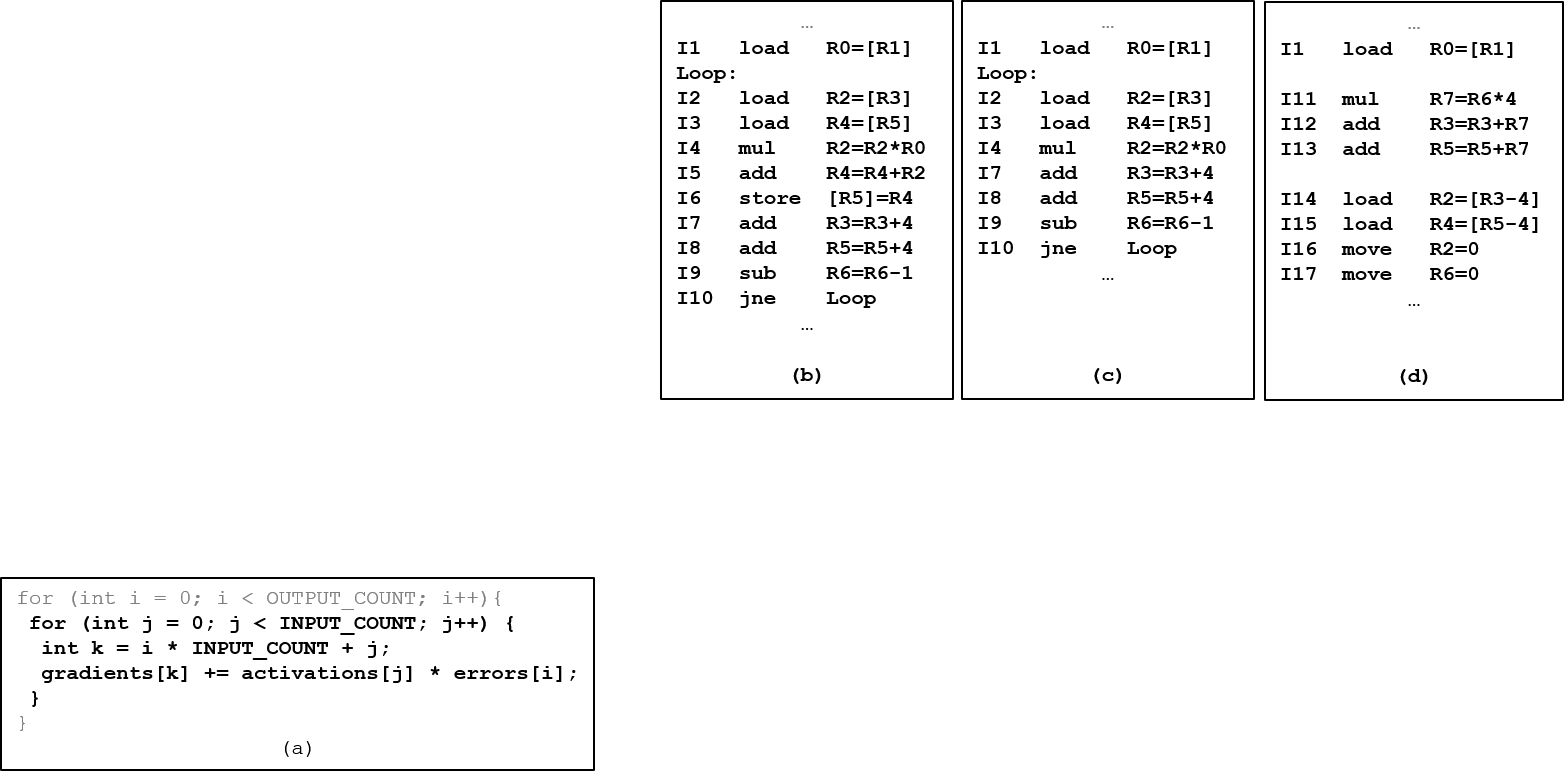
\includegraphics[width=.9\columnwidth]{Figures/gradient_source_code.png}
\caption{Code snippet for computing weight gradients.}
 \label{fig:gradient_source_code}
 \end{figure}

\subsection{Optimization Opportunities in Training Codes}

We motivate our hardware optimizations for sparse data and computations in training using a performance-critical kernel for computing synaptic weight gradients during back-propagation.  Figure~\ref{fig:gradient_source_code} illustrates a simplified version of this kernel\footnote{Our approach applies to the vector forms (e.g., SIMD) of these kernels, but we use the simple forms in our discussion for convenience.}.   Weight gradients are computed by the inner product of the activation and error vectors.  Given the sparsity in training data and computations, we observe that a promising optimization for this kernel is to skip multiply and addition operations if \emph{inputActivations[i]} or \emph{outputErrors[j]} is zero.  Moreover, the inner loop can be skipped entirely if \emph{errors[j]} is zero.  These optimizations are also effective for other performance-critical kernels of training, e.g., feed-forward evalution. 

Although these optimizations could be implemented in software by checking the data values for zero, that approach has a couple of practical limitations.   First, it requires software changes which might not be possible for existing binaries.   Second, the required software checks incur both compute and memory overheads, which could be significant and outweigh the optimization benefits.  For example, checking \emph{inputActivations[i]} and checking \emph{outputErrors[j]} have different performance impacts.  Checking \emph{outputErrors[j]} is likely to be beneficial because it can be done outside the inner loop, and helps to skip large amounts of computation. In contrast, checking \emph{inputActivations[i]} will likely hurt performance because it occurs inside the inner loop, and can save only a small amount of computation. Our hardware optimizations  avoid these limitations.  We compare the performance benefits of software and hardware  approaches in our evaluation. 



